\noindent
% CỘT LỀ TRÁI (MARGIN COLUMN)
\begin{minipage}[t]{0.26\textwidth}
  \vspace{0pt}%
  % Ảnh Tháp CN ở Toronto (được trim phần đáy để ẩn chú thích tiếng Anh cũ, dòng tác quyền gốc đã có sẵn trên ảnh)
  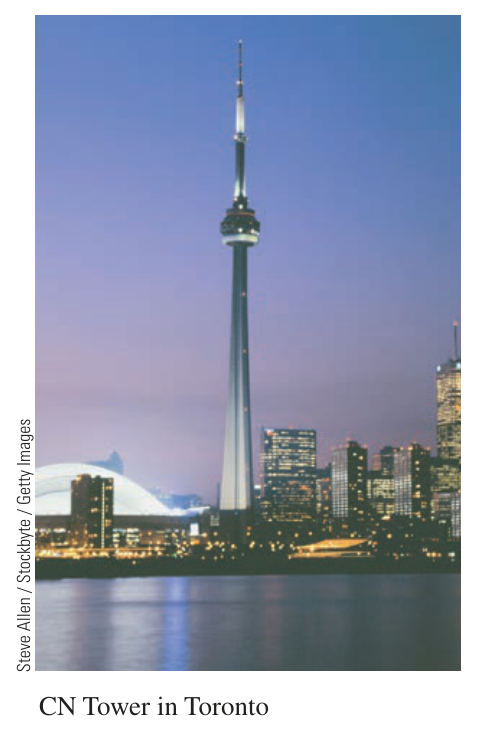
\includegraphics[width=\linewidth, trim=0 13pt 0 0, clip]{images/p0116_fig1.png}
  
  \vspace{4pt}
  {\fontsize{8.5pt}{10.5pt}\selectfont\textsf{Tháp CN ở Toronto}\par}

  % Khoảng cách dóng hàng chính xác để Hình 6 ngang hàng với bảng tính và đoạn văn liên quan
  \vspace{3.6cm}
  % Đồ thị minh họa cát tuyến và tiếp tuyến (Hình 6)
  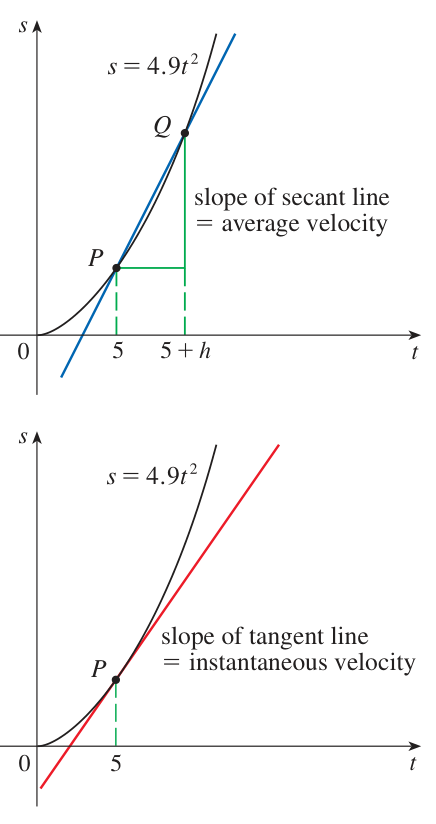
\includegraphics[width=\linewidth]{images/p0116_fig2.png}
  
  \vspace{4pt}
  {\fontsize{9pt}{11pt}\selectfont\textbf{\textsf{HÌNH 6}}}
\end{minipage}%
\hfill
% CỘT NỘI DUNG CHÍNH (MAIN COLUMN)
\begin{minipage}[t]{0.70\textwidth}
  \vspace{0pt}%
  {\textbf{\textsf{\color{stewartcyan}VÍ DỤ 3}}}\quad
  Giả sử một quả bóng được thả rơi từ đài quan sát trên cao của Tháp CN ở Toronto, cách mặt đất $450\text{ m}$. Hãy tìm vận tốc của quả bóng sau $5$ giây.

  \vspace{2pt}
  {\textbf{\textsf{\color{stewartcyan}LỜI GIẢI}}}\quad
  Khó khăn trong việc tìm vận tốc tức thời tại thời điểm $5$ giây là chúng ta đang làm việc với một thời điểm duy nhất ($t = 5$), do đó không có khoảng thời gian nào được tính đến. Tuy nhiên, ta có thể xấp xỉ đại lượng cần tìm bằng cách tính vận tốc trung bình trong khoảng thời gian rất ngắn bằng một phần mười giây từ $t = 5$ đến $t = 5{,}1$:
  \begin{align*}
    \text{vận tốc trung bình} &= \frac{\text{độ thay đổi vị trí}}{\text{thời gian trôi qua}} \\[6pt]
    &= \frac{s(5{,}1) - s(5)}{0{,}1} \\[6pt]
    &= \frac{4{,}9(5{,}1)^2 - 4{,}9(5)^2}{0{,}1} = 49{,}49\text{ m/s}
  \end{align*}

  Bảng sau đây thể hiện kết quả của các phép tính tương tự đối với vận tốc trung bình qua các khoảng thời gian ngắn dần liên tiếp.

  \vspace{2pt}
  \begin{center}
    \renewcommand{\arraystretch}{1.25}
    \fontsize{9pt}{11pt}\selectfont
    \begin{tabular}{|>{\centering\arraybackslash}m{3.2cm}|>{\centering\arraybackslash}m{3.8cm}|}
      \hline
      \rowcolor{tableheader}
      \textsf{Khoảng thời gian} & \textsf{Vận tốc trung bình (m/s)} \\
      \hline
      $5 \leqslant t \leqslant 5{,}1$   & $49{,}49$ \\
      $5 \leqslant t \leqslant 5{,}05$  & $49{,}245$ \\
      $5 \leqslant t \leqslant 5{,}01$  & $49{,}049$ \\
      $5 \leqslant t \leqslant 5{,}001$ & $49{,}0049$ \\
      \hline
    \end{tabular}
  \end{center}
  \vspace{2pt}

  Dường như khi ta rút ngắn khoảng thời gian, vận tốc trung bình ngày càng tiến gần hơn đến $49\text{ m/s}$. \textbf{Vận tốc tức thời} khi $t = 5$ được định nghĩa là \textit{giá trị giới hạn} của các vận tốc trung bình này trong các khoảng thời gian ngày càng ngắn hơn bắt đầu tại $t = 5$. Do đó, có vẻ như vận tốc (tức thời) sau $5$ giây là $49\text{ m/s}$.\hfill{\color{stewartcyan}$\blacksquare$}

  \vspace{4pt}
  Bạn có thể nhận thấy rằng các phép tính được dùng để giải quyết bài toán này rất giống với các phép tính đã dùng trước đó trong mục này để tìm tiếp tuyến. Trên thực tế, có một mối liên hệ chặt chẽ giữa bài toán tiếp tuyến và bài toán vận tốc. Nếu chúng ta vẽ đồ thị của hàm khoảng cách của quả bóng (như trong Hình 6) và xét các điểm $P(5;\, 4{,}9(5)^2)$ và $Q(5 + h;\, 4{,}9(5 + h)^2)$ trên đồ thị, thì hệ số góc của cát tuyến $PQ$ là
  \[
    m_{PQ} = \frac{4{,}9(5 + h)^2 - 4{,}9(5)^2}{(5 + h) - 5}
  \]
  đại lượng này đúng bằng vận tốc trung bình trong khoảng thời gian $[5;\, 5 + h]$. Do đó, vận tốc tại thời điểm $t = 5$ (giới hạn của các vận tốc trung bình này khi $h$ dần tiến về $0$) phải bằng hệ số góc của tiếp tuyến tại $P$ (giới hạn hệ số góc của các cát tuyến).

  \vspace{2pt}
  Các Ví dụ 1 và 3 cho thấy để giải quyết các bài toán tiếp tuyến và vận tốc, chúng ta phải có khả năng tìm giới hạn. Sau khi nghiên cứu các phương pháp tính giới hạn trong năm mục tiếp theo, chúng ta sẽ quay trở lại với các bài toán tìm tiếp tuyến và vận tốc trong Mục 2.7.
\end{minipage}
